%
\section{Results \& Discussion}\label{sec:Results & Discussion}
%
In this chapter, we summarize the results obtained from our experiments. Our experiment is mainly focused on automating the open-source software discovery and finding a suitable vulnerability database for vulnerability analysis.

\subsection{Open-Source Software Discovery}
As defined previously, the scanner has to scan \acs{OSS} components from different application framework projects. It means that the scanner should have a standard output function even if it scans different projects. In this experiment, first, we have tried using manual scrapping to understand how the \acs{OSS} components can be identified and where it is registered inside the project. Manual scrapping will be an easy solution if it is a small project, but it will be time-consuming if performed in a large scale project. Figure ~\ref{fig:laravel}, ~\ref{fig:ruby}, ~\ref{fig:gradle}, ~\ref{fig:django}, ~\ref{fig:pom} and ~\ref{fig:dotnet} shows where exactly the OSS components are registered in the project. With the help of manual scrapping from these files, we can extract the component name and version by traditional copy \& pasting technique. Then we have to search vulnerability information of each component in the vulnerability database. Therefore manual scrapping for big projects will be a time-consuming task, and also there is a possibility for human errors.
\begin{figure}[h!]
	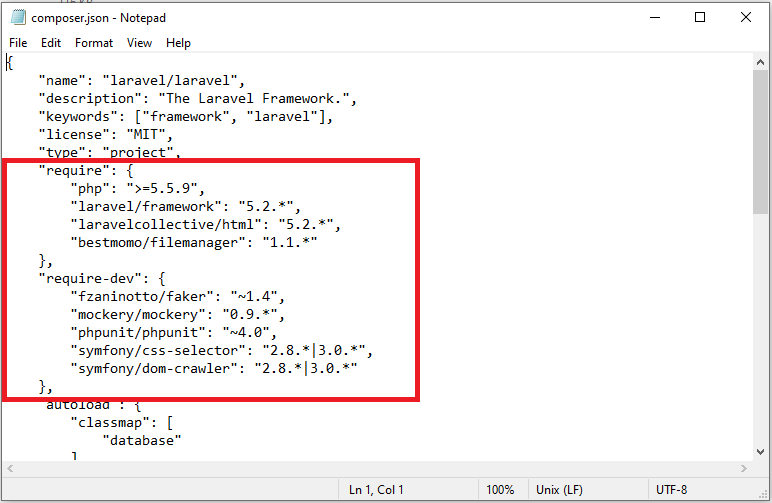
\includegraphics[width=15cm]{includes/laravel.PNG}
	\centering
	\caption{Laravel project config file}
	\label{fig:laravel}
\end{figure}
\begin{figure}[H]
	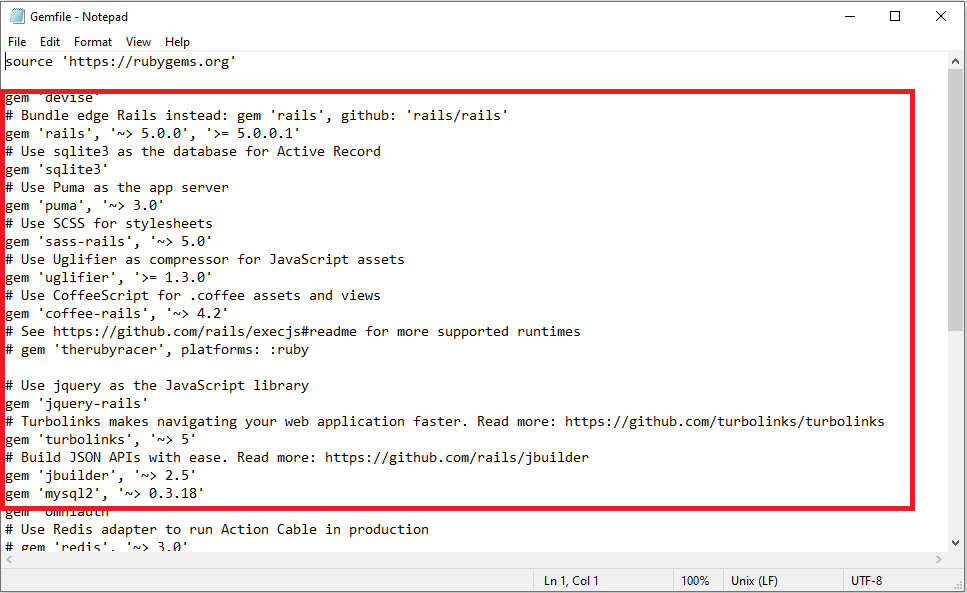
\includegraphics[width=15cm]{includes/ruby.PNG}
	\centering
	\caption{Ruby on Rails project config file}
	\label{fig:ruby}
\end{figure}
\begin{figure}[H]
	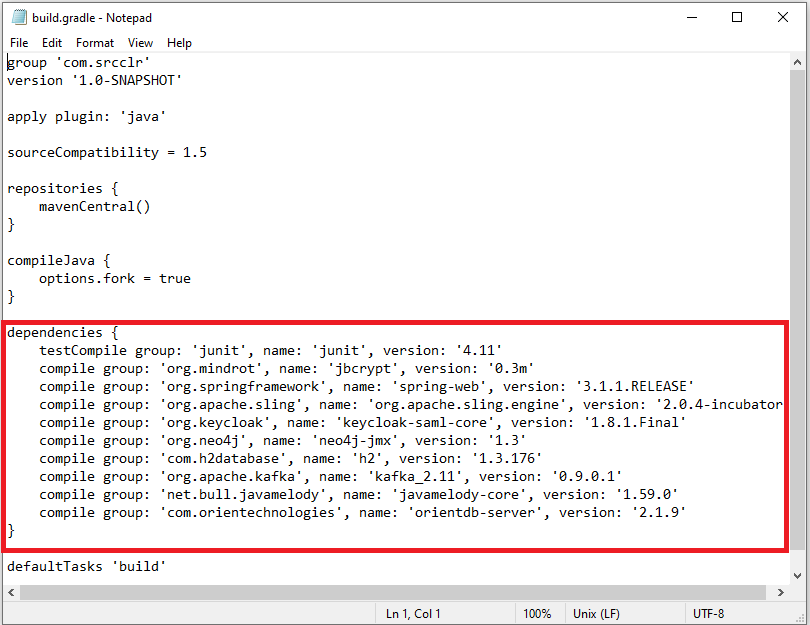
\includegraphics[width=15cm]{includes/gradle.PNG}
	\centering
	\caption{Gradle project config file}
	\label{fig:gradle}
\end{figure}
\begin{figure}[H]
	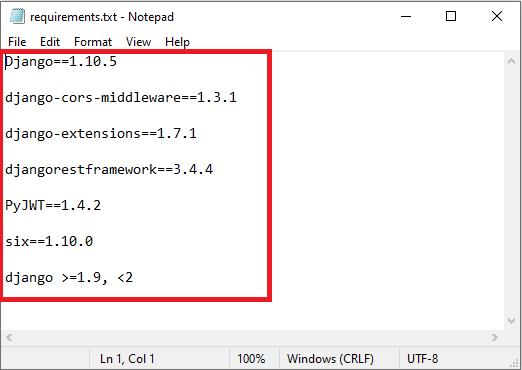
\includegraphics[width=15cm]{includes/django.PNG}
	\centering
	\caption{Django project config file}
	\label{fig:django}
\end{figure}
\begin{figure}[H]
	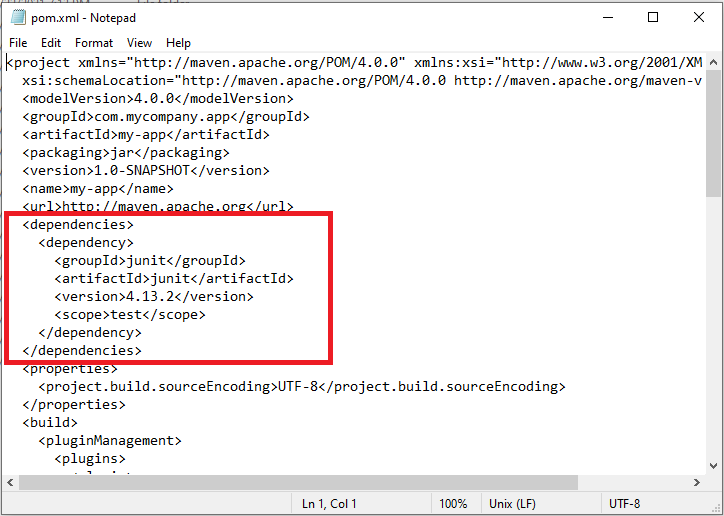
\includegraphics[width=15cm]{includes/pom.PNG}
	\centering
	\caption{Maven project config file}
	\label{fig:pom}
\end{figure}
\begin{figure}[H]
	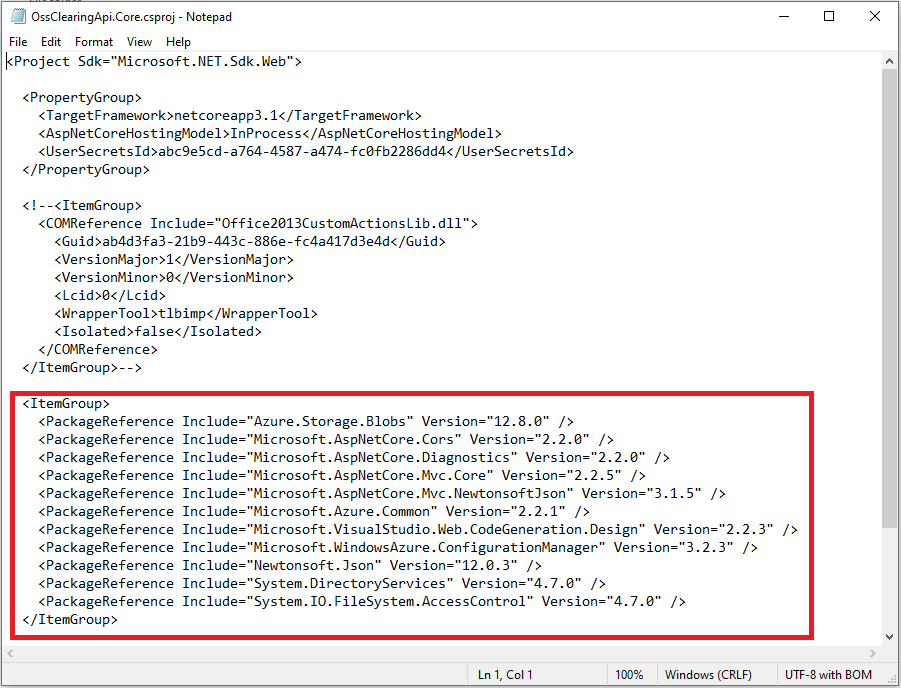
\includegraphics[width=15cm]{includes/dotnet.PNG}
	\centering
	\caption{Dotnet project config file}
	\label{fig:dotnet}
\end{figure}

After experimenting the manual scraping, we tried automating the process by using Automated scraping methods. \acs{DOM} parsing and text pattern matching methods are used for automated extraction. The main reason to use these two scraping methods is that the scanning takes place on the client-side. These two methods of scrapping can be achieved by using the Angular framework. For projects like Dotnet, Gradle, Laravel and Maven \acs{DOM} parsing methods are used because the config files of these projects are \acs{XML} and \acs{JSON} files. The text pattern matching methods are used for Django and Ruby on Rails projects. Finally, by using these two scraping methods, a generic function is created to give a final output as a \acs{JSON} object. Figure ~\ref{fig:clientOutput} will illustrate the extracted component from the Ruby on Rails project within the browser. Along with the component name and version, we have also shown from which file it is extracted. 
\newpage
\begin{figure}[H]
	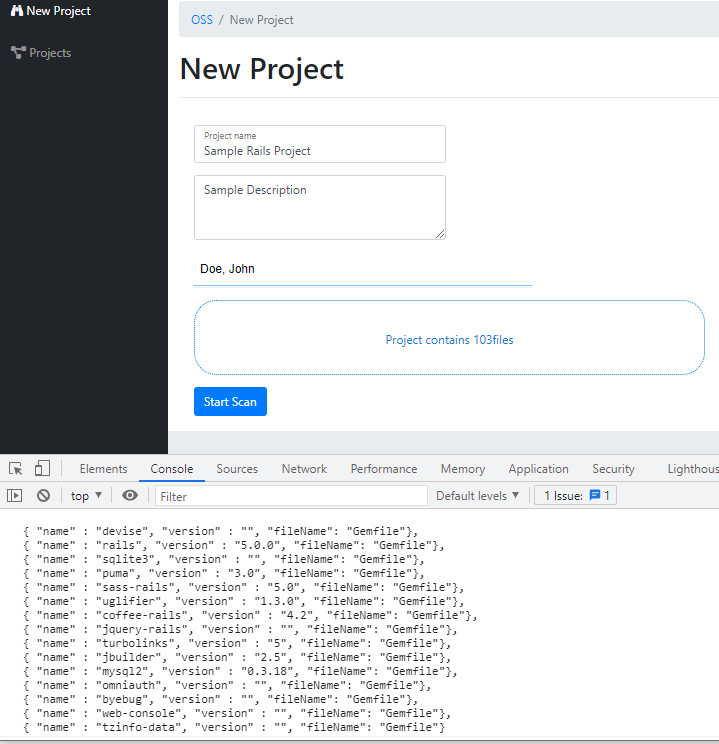
\includegraphics[width=15cm]{includes/clientOutput.PNG}
	\centering
	\caption{\acs{OSS} component name and version extraction from Ruby on Rails project}
	\label{fig:clientOutput}
\end{figure}

\subsection{Vulnerability Databases}
After scraping the component name and its version, the following process is to find the vulnerabilities of each \acs{OSS} component. Before starting the process, we must first find a reliable vulnerability database with programmatic access to automate the process. The IBM X-Force was the first database I found, and apart from the regular user interface access, it also has programmatic access like API services. Though IBM X-Force has all the utilities to automate the process, it is accessible only for non-commercial use, not for commercial purposes. The following database, which we experimented with, is CERT/CC, but before exploring it further, the database has only user interface access and no programmatic access.
\paragraph{}
The next database was Bugtraq(Security Focus), but unfortunately, it has been shut down from January 31st 2021\cite{Cat2021}. Still, the website is live with old data, and it can be used for manual searching. On top of the, accessing a shut downed service will open for other security threats. All three databases mentioned above uses \acs{CVE} dictionary to search and register the vulnerabilities. Considering the requirements like secured, reliable, programmatic access and commercial use, the \acs{NVD} database is a suitable fit for searching vulnerability. The \acs{NVD} database is completely open-source, and we can use it for both commercial and non-commercial use. When comparing \acs{NVD} with IBM X-Force, the key advantage is that it is completely open-source. The \acs{NVD} database has individual API documentation for both \acs{CVE} and \acs{CPE}. Therefore the \acs{OSS} component can be verified with the help of \acs{CPE}. Like IBM X-Force, the \acs{NVD} database also give \acs{CVSS} scores for each component so that the users will find it easy to assess the \acs{OSS} component. Figure ~\ref{fig:nvdOutput} shows the \acs{CVSS} both V2 and V3 scores of PyJwt 0.3.2 \acs{OSS} component vulnerability information. 
\begin{figure}[H]
	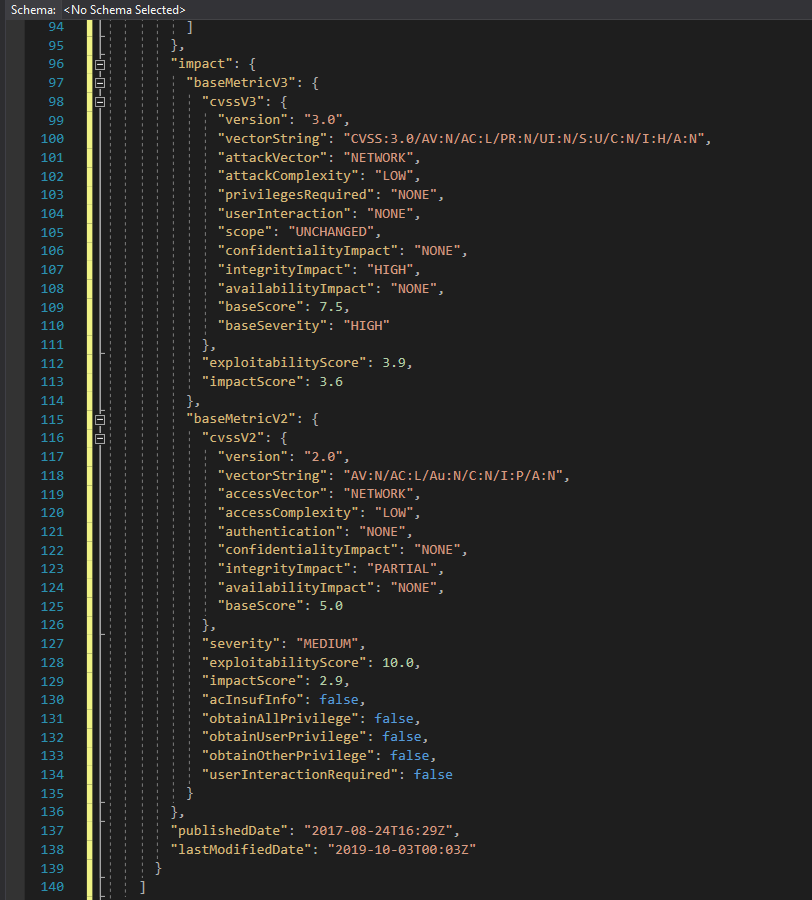
\includegraphics[width=15cm]{includes/nvdOutput.PNG}
	\centering
	\caption{Vulnerability information of PyJwt 0.3.2 component from \acs{NVD} database}
	\label{fig:nvdOutput}
\end{figure}

\subsection{Vulnerability Report:}
The report will be ready to download once the vulnerability assessment is over. The main task of this module is to give a simple report of the \acs{OSS} component discovered and its vulnerability information. The report will have both \acs{CVSS} V2 and V3 properties so that the user can assess the component based on their requirements. The \acs{CVE} and \acs{CPE} id will also be in the report. Therefore the user can look up further information externally if it is needed. This report will not make any decisions on behalf of the user. It will just share the vulnerability details of each \acs{OSS} component. Based on the vulnerability information, the user can decide whether to keep the OSS component or move to the next possible version. Figure ~\ref{fig:nvdOutput} will illustrate how the report indicates vulnerability information of each \acs{OSS} component.
\begin{figure}[H]
	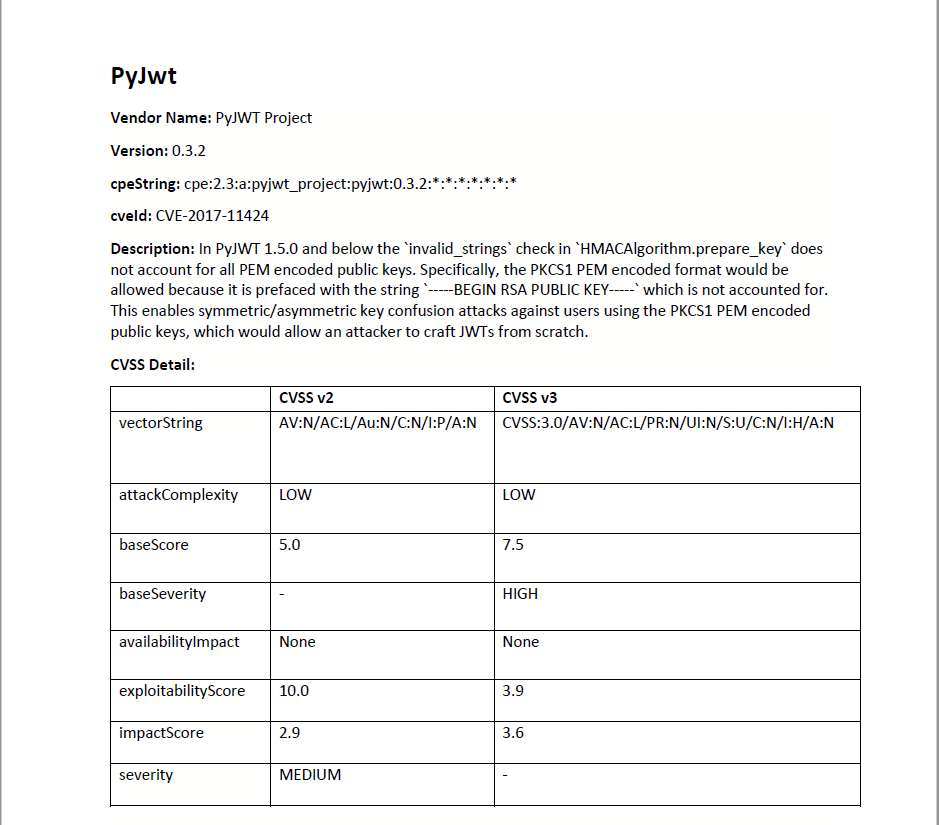
\includegraphics[width=15cm]{includes/report.PNG}
	\centering
	\caption{Sample Report of PyJwt 0.3.2 component from \acs{NVD} database}
	\label{fig:report}
\end{figure}